
\section{Архитектура и модули системы} % (fold)
\label{sec:arch_and_mod}

Разработанное программное обеспечение представляет из себя библиотеку кода написанную на языке ruby.
Библиотека предназначена лексической и функциональной обфускации исходных кодов, написанных на языке VHDL.
Библиотeка состоит из следующих компонентов:
\begin{itemize}
\item лексический анализатор(лексер);
\item синтаксический анализатор(парсер);
\item обфускатор;
\end{itemize}
Поскольку в данной библиотеке используется синтаксический анализатор LALR-типа, действия интегрируются прямо в грамматику языка. Из этого следует, что обфускатор, хоть и является отдельным компонентом, представленным в виде набора классов, всё же интегрирован в синтаксический анализатор. Процесс работы ПС представлен на рисунке~\ref{fig:arch_and_mod::abstract_flow}.
\afterpage{
  \begin{landscape}
  \thispagestyle{lscape}
  \begin{figure}[t!]
  \centering
    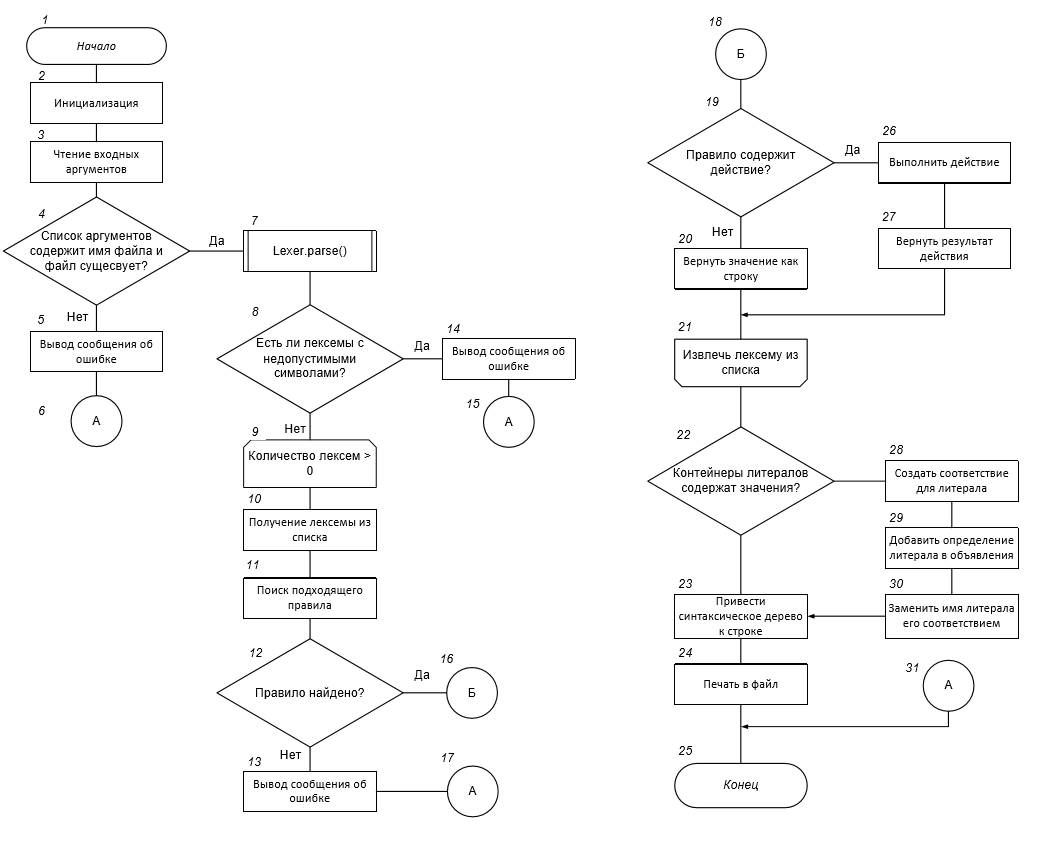
\includegraphics[scale=0.65]{program_flow.png}
    \caption{ Схема работы программы }
    \label{fig:arch_and_mod::abstract_flow}
  \end{figure}
  \end{landscape}
}

\subsection{Лексический анализатор}
\label{sub:arch_and_mod:lexer}

Так как в дипломном проекте используется синтаксический анализ исходного кода, то, очевидно, для этого анализа должна быть часть, отвечающая за процесс аналического разбора входной последовательности символов. Слово <<лексический>> в традиционном смысле означает <<относящийся к словам>>. С точки зрения языка программирования, слова являются объектами, такими как имена переменных, числа, ключевые слова и т.д. Такие слова традиционно называются <<токенами>>~\cite{basic_compiler_design}.

Лексический анализатор, или \textit{лексер}, принимает в качестве входных параметров строку символов, и разделяет эту строку на лексемы. Кроме того, он отфильтровывает все, что разделяет токены, то есть элементы разметки символов (пробелы,переводы строк т.п.) и комментарии.

Основная цель лексического анализа --- упростить процесс последующего синтаксического анализа. В теории, работа, которая проводится во время лексического анализа может
составлять неотъемлемую часть синтаксического анализа, так и в простых системах это действительно почти всегда справедливо. Тем не менее, есть основания для разделения синтаксического и лексического анализа:
\begin{itemize}
\item
  эффективность: Лексический анализатор может делать простые операции быстрее, чем это делает обычный парсер, кроме того, размер системы, которая разделена на две части, может
  быть меньше, чем в объединенной системе;
\item
  модульность: Синтаксическое описание языка не должно быть загромождено мелкими лексическими деталями, такими как пробелы и комментарии;
\item
  традиция: языки часто проектируются с отдельными лексическими и синтаксическими анализаторами, а также стандарты таких языков обычно разделяют лексические и синтаксические элементы;
\end{itemize}
Схема работы лексического анализатора, представленного в ПС, изображена на рисунке \ref{fig:arch_and_mod::lexer_flow}

\begin{figure}[!htb]
  \centering
  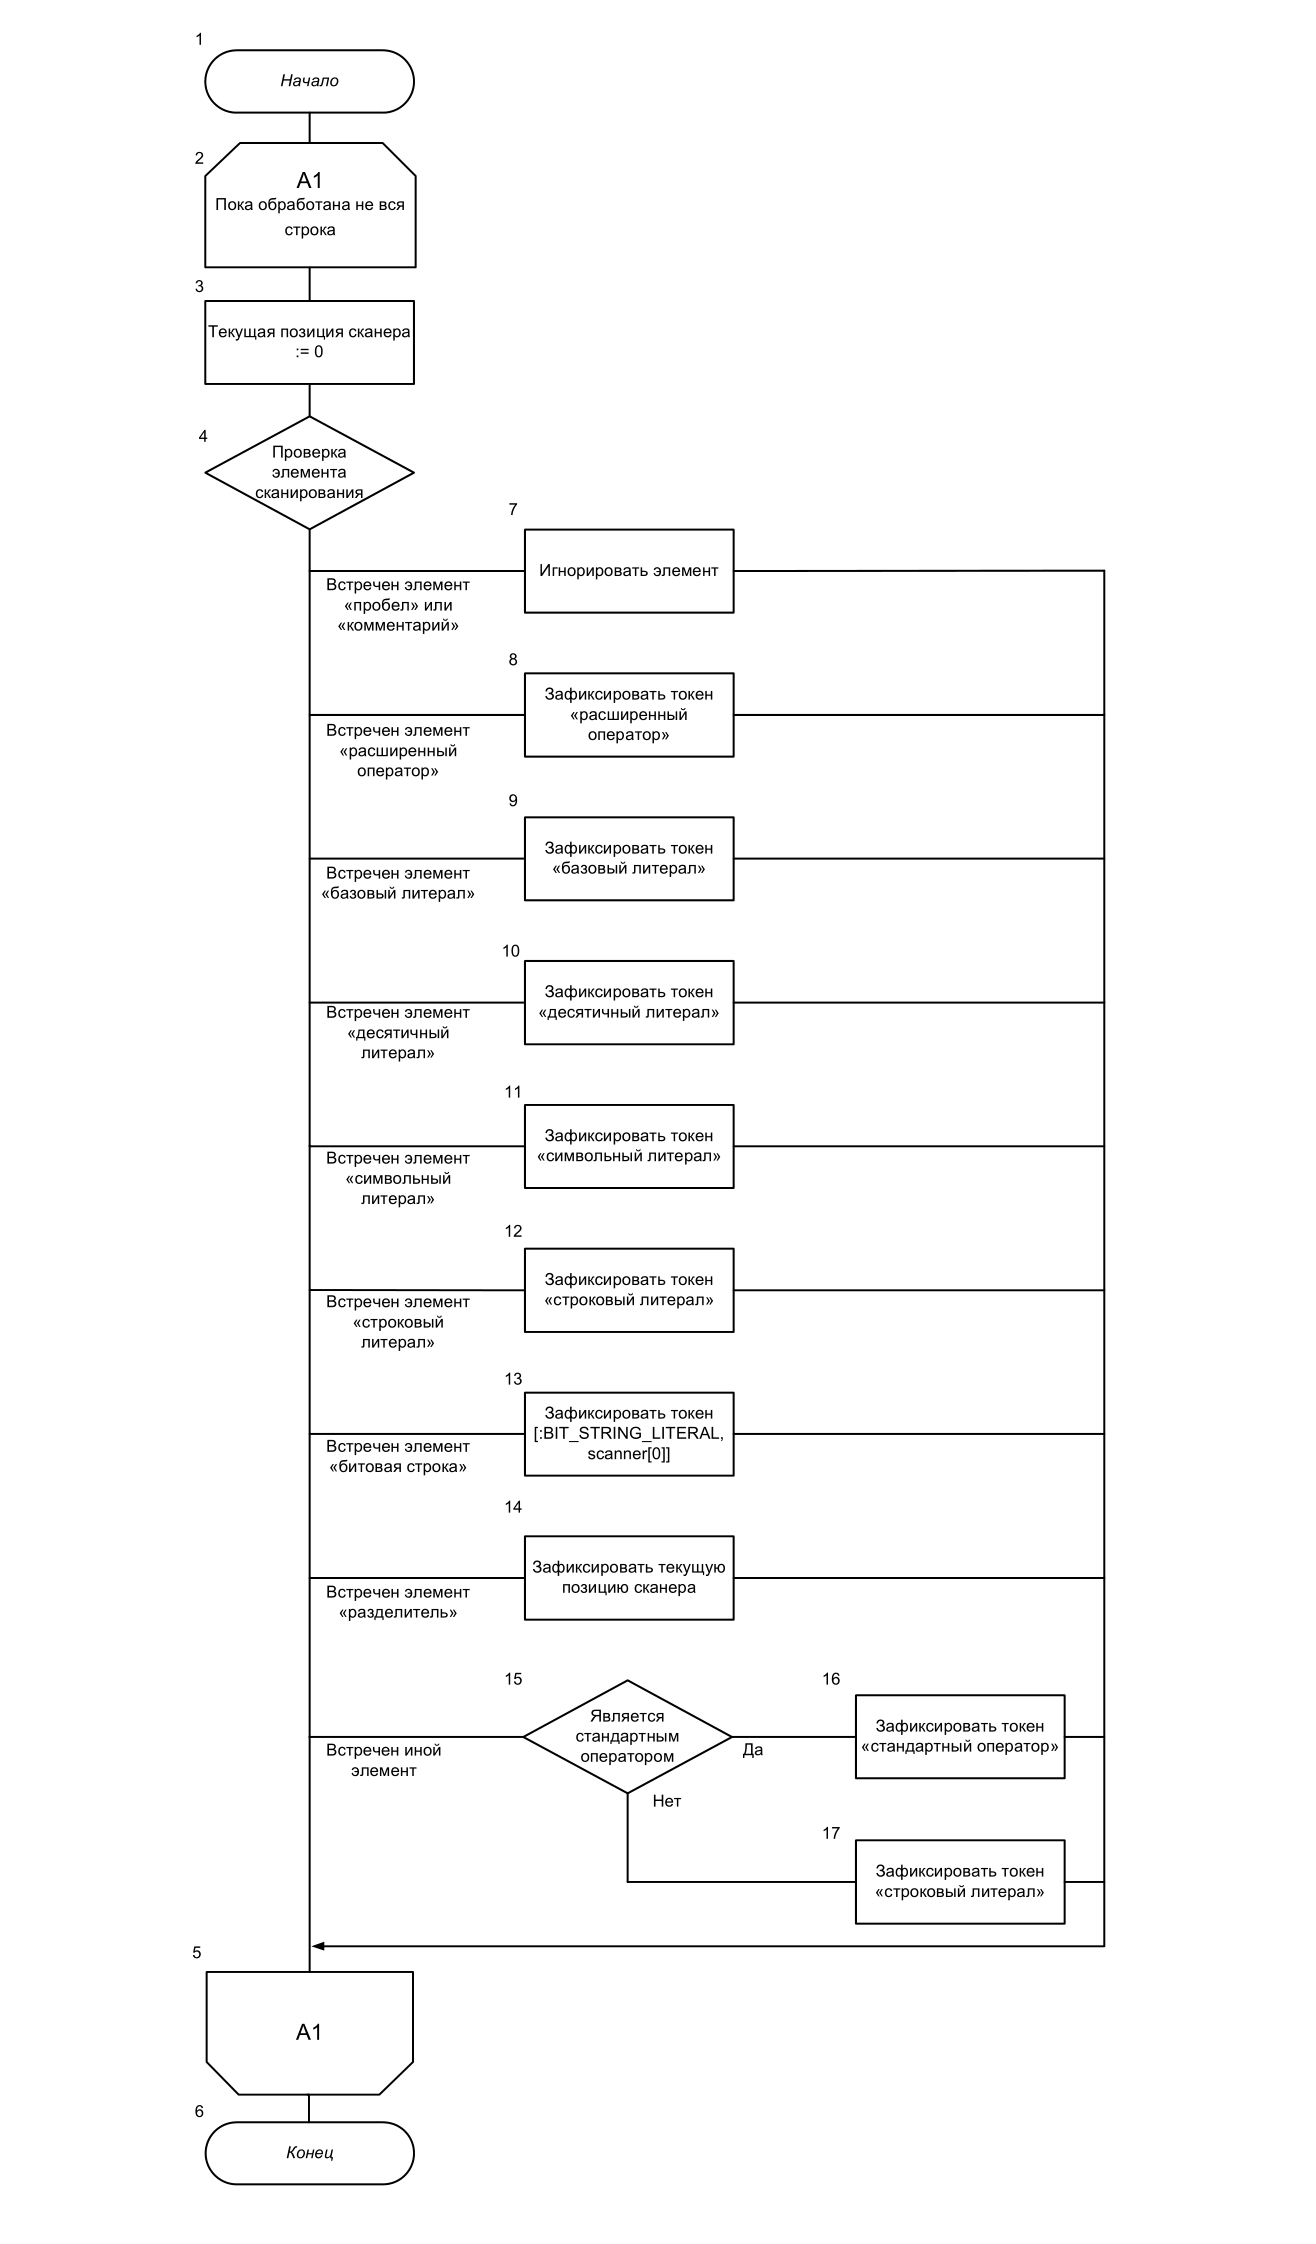
\includegraphics[scale=0.38]{lexer_flow.png}
  \caption{ Схема работы лексера }
  \label{fig:arch_and_mod::lexer_flow}
  \clearpage
\end{figure}



\subsubsection{Регулярные выражения}~
\label{sec:arch_and_mod:regex}
Основу лексера, представленного в ПС, составляют регулярные выражения: алгебраическая нотация для описания наборов строк~\cite{regular_expressions_tutorial}.

Множество всех целочисленных констант или множество всех имен переменных представляют собой наборы строк, где отдельные буквы берутся из определенного алфавита. Такой набор
строки называется \textit{языком}. Для целых чисел, алфавит состоит из цифр 0-9 и для имен переменных алфавит содержит буквы и цифры (и, возможно, некоторые из них
другие символы, такие как подчеркивание). При заданном алфавите, мы будем описывать наборы строк и обычные выражения. Алгебраическая нотация является компактной и легкой для понимания и использования людьми формой представления. Идея заключается в том, что регулярные выражения, которые описывают простые наборы строк могут быть объединены, чтобы формировать регулярные выражения, которые описывают более сложные наборы строк.

Регулярные выражения разбивают входной поток символов на части, которые затем анализируются, и трансфомируются в токены. Лексер считывает поток символов и останавливается только при встрече определенного символа, называемого \textit{разделителем}. Эти символы уникальны для каждого языка и определены его грамматикой. Разделитель, используемый в программе, а также его использование, приведены в листинге \ref{lst:arch_and_mod:delimiter_usage}:
\begin{lstlisting}[language=Ruby, style=rubystyle,caption={Определение и использование разделителя}, label=lst:arch_and_mod:delimiter_usage]
DELIMITER = '=>|\*\*|:=|\/=|>=|<=|<>|\Z|[&\'()*+,-.\/\:;<=>|\[\]]'
DELIMITER_RE = /(?:#{DELIMITER})/

def parse(str)
  .
  .
  .

  scanner.check_until(/\s|#{DELIMITER}/)
  v = scanner.pre_match[before..-1]
  scanner.pos += v.size
  case v
  when /^abs$/i then
    [:ABS, "abs"]
  when /^access$/i then

  .
  .
  .
end
\end{lstlisting}

Помимо разделителя, в лексере также присутствуют другие регулярные выражения, которые отвечают за определение токены. Эти регулярные выражения и их использование приведены в листинге~\ref{lst:arch_and_mod:literal_usage}:
\begin{lstlisting}[language=Ruby, style=rubystyle,caption={Определение и использование регулярных выражений для опознавания токена}, label=lst:arch_and_mod:literal_usage]
UPPERCASE_LETTERS = 'A-Z'
DIGITS = '0-9'
SPECIAL_CHARS = '\s#&\'\(\)*+,-\.\/\:\;<=>\[\]_|'
SPACE_CHARS = ' '

BASIC_GRAPHIC_CHAR = "#{UPPERCASE_LETTERS}#{DIGITS}#{SPECIAL_CHARS}#{SPACE_CHARS}"
GRAPHIC_CHARS = "#{BASIC_GRAPHIC_CHAR}#{LOWERCASE_LETTERS}#{OTHER_SPECIAL_CHARS}"
BASIC_CHARS = "#{BASIC_GRAPHIC_CHAR}#{FORMAT_EFFECTOR}"

BASIC_IDENT_RE = /[A-Za-z][A-Za-z0-9_]*/
EXTENDED_IDENT_RE = /\\([#{GRAPHIC_CHARS}]+)\\/

INTEGER = '[0-9][0-9_]*'
EXPONENT = 'E[+-]?[0-9][0-9_]*'
BASED_INTEGER  = '[0-9A-Za-z][0-9A-Za-z_]*'
BIT_VALUE = '[0-9A-Za-z][0-9A-Za-z_]*'

DECIMAL_LITERAL_RE = /#{INTEGER}(?:\.#{INTEGER})?(?:#{EXPONENT})?/
BASED_LITERAL_RE = /#{INTEGER}#(?:#{BASED_INTEGER})(?:\.#{BASED_INTEGER})?#(?:#{EXPONENT})?/
CHAR_LITERAL_RE = /'([#{GRAPHIC_CHARS}])'/
STRING_LITERAL_RE = /"([#{GRAPHIC_CHARS}]*)"/
BIT_STRING_LITERAL_RE = /[BOX]"#{BIT_VALUE}"/
COMMENT_RE = /--.*[\r\n]*/
.
.
.
@tokens = s.collect_token{|scanner|
  case
  when scanner.skip(/\s+/)
    # ignore
  when scanner.skip(COMMENT_RE)
    # ignore
  when scanner.scan(EXTENDED_IDENT_RE)
    [:EXTENDED_IDENTIFIER, scanner[1]]
  when scanner.scan(BASED_LITERAL_RE)
    [:BASED_LITERAL, scanner[0]]
  when scanner.scan(DECIMAL_LITERAL_RE)
    [:DECIMAL_LITERAL, scanner[0]]
  when scanner.scan(CHAR_LITERAL_RE)
    [:CHARACTER_LITERAL, scanner[1]]
  when scanner.scan(STRING_LITERAL_RE)
    [:STRING_LITERAL, scanner[1]]
  when scanner.scan(BIT_STRING_LITERAL_RE)
    [:BIT_STRING_LITERAL, scanner[0]]
  when scanner.scan(DELIMITER_RE)
    [scanner[0], scanner[0]]
end
\end{lstlisting}
После того, как встречен разделитель, лексер с помощью регулярных выражений определяет тип лексемы, и если она не является литералом(строковым, символьным, числовыми), проверяется принадлежность строки к набору базовых операторов языка:

\begin{lstlisting}[language=Ruby, style=rubystyle,caption={Проверка принадлежности части строки базовой конструкции языка}]
  .
  .
  .
  before = scanner.pos
  scanner.check_until(/\s|#{DELIMITER}/)
  v = scanner.pre_match[before.0]
  scanner.pos += v.size
  case v
  when /^abs$/i then
    [:ABS, "abs"]
  when /^access$/i then
    [:ACCESS, "access"]
  when /^after$/i then
    [:AFTER, "after"]
  when /^alias$/i then
    [:ALIAS, "alias"]
  when /^all$/i then
    [:ALL, "all"]
  when /^and$/i then
    [:AND, "and"]
  when /^arch$/i then
    [:ARCH, "arch"]
  when /^architecture$/i then
    [:ARCHITECTURE, "architecture"]
  when /^array$/i then
    [:ARRAY, "array"]
  .
  .
  .
end
\end{lstlisting}
Сама лексема представлена как массив, состоящий из 2 элементов: тип лексемы, и ее значение. Пример различных лексем приведен в листинге \ref{lst:arch_and_mod:lexem_definition}:
\begin{lstlisting}[language=Ruby, style=rubystyle,caption={Различные типы лексем}, label=lst:arch_and_mod:lexem_definition]
  .
  .
  .
  when /^xnor$/i then
    [:XNOR, "xnor"]
  when /^xor$/i then
    [:XOR, "xor"]
  else
    [:BASIC_IDENTIFIER, v]
  .
  .
  .
\end{lstlisting}

Данный набор лексем более чем достаточен для исчерпывающего описания языка VHDL. Использование лексера сильно упрощает работу синтаксического анализатора и добавляет ему гибкости, что позволяет расширять его функциональность.
\subsection{Синтаксический анализатор}
\label{sub:arch_and_mod:parser}
Следующий за лексическим анализом шаг --- синтаксический анализ или \textit{парсинг}.

Парсинг --- это процесс структурирования линейного представления в соответствии с заданной грамматикой. <<Линейное представление>> может быть предложением, исходным кодом программы, последовательностью геологических слоев, звуковым, файлом, короче говоря, любой линейной последовательностью, в которой предыдущие элементы некоторым способом предопределяют следующий элемент.

В дополнение к поиску структуры входного текста, синтаксический анализ должен также отвергать недействительные тексты, сообщая о синтаксических ошибках. Поскольку синтаксический анализ имеет менее локальный характер, для него требуются более продвинутые методы. В нашем случае используется та же базовая стратегия: нотация, пригодная для чтения человеком, трансформируется в машинную низкоуровневую нотацию, которая подходит для эффективного выполнения. Этот процесс называется генерацией синтаксического анализатора.

Нотация которая используется для манипуляций человека является контекстно-свободной грамматикой, которая является рекурсивным обозначением для описания наборов строк и наложения структуры на каждую такую строки. Эти нотации могут в некоторых случаях быть переведены непосредственно в рекурсивные программы, но часто бывает удобнее перевести их в конечный автомат стекового типа. Они похожи на конечный автомат, используемый для лексического анализа, но они могут дополнительно использовать стек, который позволяет считать и находить соответствия вне локального контекста.
\subsubsection{Контексто-независимые грамматики}~
\label{sub:arch_and_mod:grammars}

Подобно регулярным выражениям, контекстно-независимые грамматики описывают наборы строк, то есть \textit{языки}. Кроме того, контекстно-независимая грамматика также определяет структуру над строками в определяемом языке. Язык определен над некоторым алфавитом, например, набор токенов, полученных с помощью лексера или набор буквенно-цифровых символов. Символы в алфавите называются \textit{терминалами}. Контекстно-независимая грамматика рекурсивно определяет несколько наборов строк. Каждый набор обозначается именем, которое называется \textit{нетерминалом}. Множество нетерминалов не пересекается с другим множеством нетерминалов. Один из нетерминалов выбирается для обозначения языка, описываемого грамматикой. Это называется стартовым символом грамматики. Множества описываются рядом продукций(production rule). Каждая продукция описывает некоторые из возможных строк, содержащихся в наборе, обозначенном нетерминалом. Продукция имеет вид
\begin{equation}
  N \rightarrow X_1...X_n
\end{equation}
\begin{explanation}
где N - нетерминал, $X_1...X_n$ - 0 или более символов, каждый из которых \\
    является или терминалом, или нетерминалом
\end{explanation}

Предполагаемый смысл этого обозначения в том, что множество обозначаемое через $N$ содержит строки, которые получаются с помощью конкатенации строк из множеств, обозначенных
$X_1...X_n$. В данном случае терминал обозначает одноэлементный набор, так же, как алфавит символов в регулярных выражениях, например:

\begin{equation}
  A \rightarrow a
\end{equation}
\begin{explanation}
описывает набор, обозначенный нетерминалом $A$, который содержит строку \\
из одного символа $a$
\end{explanation}

\begin{equation}
  A \rightarrow aA
\end{equation}
\begin{explanation}
обозначает, что множество, обозначенное как $A$, содержит все строки,\\
образованные добавлением символа $a$ в начало строки, взятой из \\ множества $a$
\end{explanation}
Можно определить  грамматику, эквивалентную регулярному выражению $a*$ с помощью двух продукций:
\begin{equation}
\begin{aligned}
  &B \rightarrow        \\
  &B \rightarrow aB
\end{aligned}
\end{equation}
\begin{explanation}
где первая продукция показывает, что пустая строка является частью \\
множества $B$.
\end{explanation}

Для каждой грамматики, существует, как правило, бесконечное число линейных представлений
("предложений"), которые могут быть представлены ей. То есть, грамматика конечного размера может соответствовать бесконечному числу предложений. Это основное преимущество грамматик
и доказательство их важности: они обобщают структуру бесконечного числа объектов определенного класса~\cite{cfg_evidence}.
Есть несколько причин, чтобы выполнить процесс парсинга. Одна из
причин вытекает из того факта, что полученная структура помогает нам обрабатывать объект
в дальнейшем. Когда мы знаем, что определенный сегмент предложения на немецком языке является предметом,
эта информация помогает в переводе предложения. После того, как структура документа обработана синтаксическим анализатором, манипулировать ей становится в разы проще.
\subsubsection{Генератор парсеров YACC}~
\label{sub:arch_and_mod:parser_generator}
Посколько разработка собственного парсера является очень затратной, было принято решение использовать генератор парсеров. Генератор парсеров --- приложение, которое генерирует исходный код LALR(1)-парсера на основе BNF грамматик. Акроним LALR расшифровывается как lookahead left-right. Цифра <<1>> означает, на сколько символов вперед смотрит анализатор. Для написания был использован адаптер YACC(yet another compiler compiler) для языка ruby --- RACC. В качестве правил использовалась модифицированная BNF грамматика для языка VHDL и уникальный набор действий для каждого правила. Пример грамматики приведен в листинге \ref{lst:arch_and_mod:yacc_rules}:
\begin{lstlisting}[language=Ruby, style=rubystyle,caption={Различные описания грамматик и действия, вызываемые при соответствии грамматики линейной последовательности}, label=lst:arch_and_mod:yacc_rules]
  .
  .
  .
abstract_literal :
  DECIMAL_LITERAL {
    result = DecimalLiteral.new(val[0]);
    LiteralRepository.add(result);
  }
  | BASED_LITERAL {result = val[0]}

access_type_definition :
  ACCESS subtype_indication {result = val}

actual_designator :
  expression {result = val[0]}
  | signal_name {result = val[0]}
  | variable_name {result = val[0]}
  | file_name {result = val[0]}
  | OPEN {result = val[0]}

expression :
  relation expression_loop0 {result = Expression.new(val.flatten); }
  | STRING_LITERAL {result = StringLiteral.new(val[0]);}
  | relation expression_loop1 {result =  Expression.new(val.flatten);}
  | relation expression_loop2 {result =  Expression.new(val.flatten);}
  | relation NAND relation {result =  Expression.new(val.flatten);}
  | relation NOR relation {result =  Expression.new(val.flatten);}
  | relation expression_loop3 {result =  Expression.new(val.flatten);}

  .
  .
  .
\end{lstlisting}
Поскольку грамматики описываются в форме Бэкуса---Наура, то эти правила могут рекурсивными:


\begin{lstlisting}[language=Ruby, style=rubystyle,caption={Пример рекурсивных правил}, label=lst:arch_and_mod:recursive_rules]
  identifier_list :
    identifier identifier_list_loop0 {result = val = IdentifierList.new(val.flatten); InitializeRepository.add(result.identifiers) }

  identifier_list_loop0 :
    ',' identifier identifier_list_loop0 {result = val - [',']}
    | {result = val}
\end{lstlisting}


Подобно другим сдвиго-сверточным анализаторам, LR-парсер ожидает сканирования следующего символа и пытается сделать свертку в некую конструкцию всех элементов на стеке. Как только найдено правило для заданных элементов, парсер немедленно сворачивает конструкцию. В примере в таблице \ref{arch_and_mod:parse_table}, литерал \textit{A} сворачивается до \textit{Значения}, а затем до \textit{Умножения} (согласно имени правила) на шагах 1-3 как только следующий(lookahead) символ <<*>>  виден, а не ждет дополнительных комманд, чтобы организовать эти части дерева. Решения, как  обрабатывать литерал \textit{A} базируются только на том, что сканнер и парсер уже видели, не принимая в расчет те элементы, что будут прочтены позднее.
Свертка реорганизует последние проанализириванные элементы непосредственно слева от следующего символа. Поэтому список проанализированных элементов является стеком. Стек растет слева-направо. Вершина стека находится левее всех и содержит старейший проанализированный фрагмент. Каждый шаг свертки действует только на крайнем правом, новейшем фрагменте.
Пример обработки выражения $A*2+1$ приведен в таблице \ref{arch_and_mod:parse_table}:

\begin{table}[ht]
  \caption{Пример разбора выражения $A*2+1$}
  \label{arch_and_mod:parse_table}
  \begin{tabular}{| >{\centering}m{0.07\textwidth}
                  | >{\centering}m{0.23\textwidth}
                  | >{\centering}m{0.2\textwidth}
                  | >{\centering}m{0.4\textwidth}|}
  \hline
  Шаг & Cтек парсера & Выражение & Сдвиг/Свертка \tabularnewline
  \hline
  0 & empty & $A*2+1$ & Cдвиг \tabularnewline
  \hline
  1 &  id  & $*2 + 1$ & Значение $\rightarrow $ id \tabularnewline
  \hline
  2 &  Value &  $*2 + 1$ & Products $\rightarrow $ Value \tabularnewline
  \hline
  3 &  Products & $*2 + 1$ & Сдвиг \tabularnewline
  \hline
  4 &  Products  * &  $2 + 1$  & Сдвиг \tabularnewline
  \hline
  5 &  Products  * int &$  + 1$  & Value $\rightarrow $ int \tabularnewline
  \hline
  6 &  Products  * Value &  $+ 1$ &  Products $\rightarrow $ Products * Value \tabularnewline
  \hline
  7 &  Products & $+ 1$  &  Sums $\rightarrow $ Products \tabularnewline
  \hline
  8 &  Sums & $+ 1$  & Сдвиг \tabularnewline
  \hline
  9 &  Sums  + &  $1$  & Сдвиг \tabularnewline
  \hline
  10 & Sums  + int &  eof &  Value $\rightarrow $ int \tabularnewline
  \hline
  11 & Sums + Value & eof &   Products $\rightarrow $ Value \tabularnewline
  \hline
  12 & Sums + Products &  eof  & Sums $\rightarrow $ Sums + Products \tabularnewline
  \hline
  13 & Sums & eof &  done \tabularnewline
  \hline
  \end{tabular}
\end{table}


На рисунке~\ref{fig:arch_and_mod::lr_example_img} представлено состояние парсера на одном из шагов.

\begin{figure}[!htb]
  \centering
  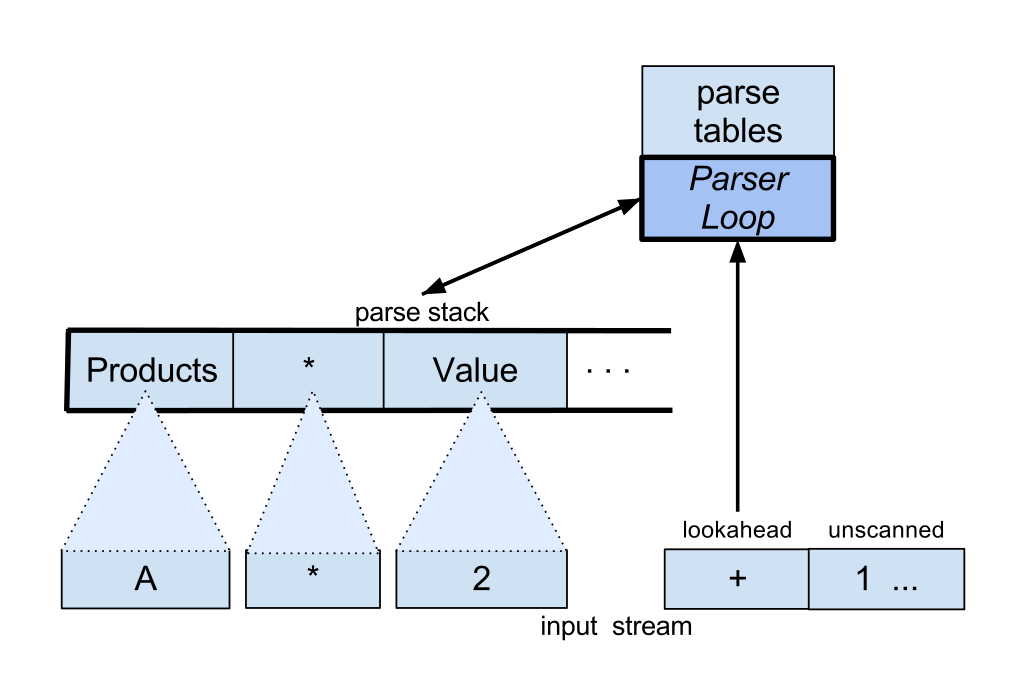
\includegraphics[scale=0.3]{parser_state.png}
  \caption{ Состояние парсера на шаге №6 }
  \label{fig:arch_and_mod::lr_example_img}
\end{figure}



\subsubsection{Абстрактное синтаксическое дерево}~
\label{sub:arch_and_mod:ast}
Каждое правило содержит действие, которое выполнится при соответствии оного. В данном ПС эти действия на построение абстрактного синтаксического дерева(Abstract syntax tree, AST), которое представляет собой структуру программы в удобном виде, с возможностью модификации узлов, что является необходимым условием для обфускации исходной последовательности.

Абстрактное синтаксическое дерево --- это конечное, помеченное, ориентированное дерево, в котором внутренние вершины сопоставлены с операторами языка программирования, а листья --- с соответствующими операндарми. Таким образом, листья являются пустыми операторами и представляют только переменные и константы~\cite{ast}.

Для языка, который описывается контекстно-независимой грамматикой, какими являются почти все языки программирования, создание абстрактного дерева в синтаксическом анализаторе является тривиальной задачей. Большинство правил в грамматике создают новую вершину, а символы в правиле становятся ребрами. Правила, которые ничего не привносят в АСД(например, группирующие правила), просто заменяются в вершине одним из своих символов. Кроме того, анализатор можешт создать полное дерево разбора и затем пройти по нему, удаляя узлы и рёбра, которые не используются в абстрактном синтаксисе, для получения АСД.

Структура АСД часто тесно связана с дизайном компилятора и его ожидаемых функций.
Основные требования включают в себя следующее:
\begin{itemize}
\item  Типы переменных должны быть сохранены, а также расположение каждого объявления в исходном коде.
\item  Порядок исполняемых операторов должен быть явно представлены и четко определен.
\item  Левая и правая компоненты бинарных операций должны храниться и правильно определены.
\item  Идентификаторы и назначенные им значения должны быть сохранены для операторов присваивания.
\end{itemize}

Некоторые операции всегда будут требовать двух элементов, таких, как два слагаемых для операции суммирования. Тем не менее, некоторые языковые конструкции требуют сколь угодно большого числа операндов, таких как списки аргументов, передаваемых программе из командной оболочки. В результате, АСД используется для представления кода, написанного на таком языке, который должен быть достаточно гибким, чтобы позволить быстрое добавление неизвестного количества детей(листьев дерева).
Еще одним желательным условием конструкции для АСД является то, что должна быть обеспечена возможность представления АСД в виде исходного кода. Исходный код, сгенерированный из АСД, должен быть достаточно похожим на оригинал по внешнему виду и идентичным в исполнении. Последнее является обязательным, так как после обфускации дерева его необходимо перевести в исходный код.

\subsection{Обфускатор}
\label{sub:arch_and_mod:grammars}

После того, как сформировано синтаксическое дерево, необходимо внести в его изменения. В данном ПС обфускатором представлен наборов классов-оболочек над примитивами языка VHDL и контейнерами литералов. Полный алгоритм работы обфускатора представлен на рисунке \ref{fig:arch_and_mod:obf_algo}.
Т.к мы используем генератор парсеров, то обфускатор инициализируется на этапе синтаксического анализа(создаются экземпляры классов, создаются соответствия между реальными именами переменных и их обфусцированными вариантами). Сам процесс обфускации реализован через определение метода \textbf{to\_s}  у классов-оболочек, что позволяет автоматически заменять имена переменных, вставлять произвольный код прямо в процессе конвертации экземпляра класса в строку:

\begin{lstlisting}[language=Ruby, style=rubystyle,caption={Определение метода перевода класса в строку для примитива component instantiation}, label=lst:arch_and_mod:wrapper_to_s]
  def to_s
    "#{@name} : #{@instantiated_unit} #{@generic_map_aspect}#{@port_map_aspect ? '' : ';'}#{@port_map_aspect}"
  end
\end{lstlisting}


\subsubsection{Контейнеры литералов}
  Контейнеры литералов представлены в виде трёх классов для различных видов литералов:
  \afterpage{
    \begin{landscape}
    \thispagestyle{lscape}
    \begin{figure}[ht]
    \centering
      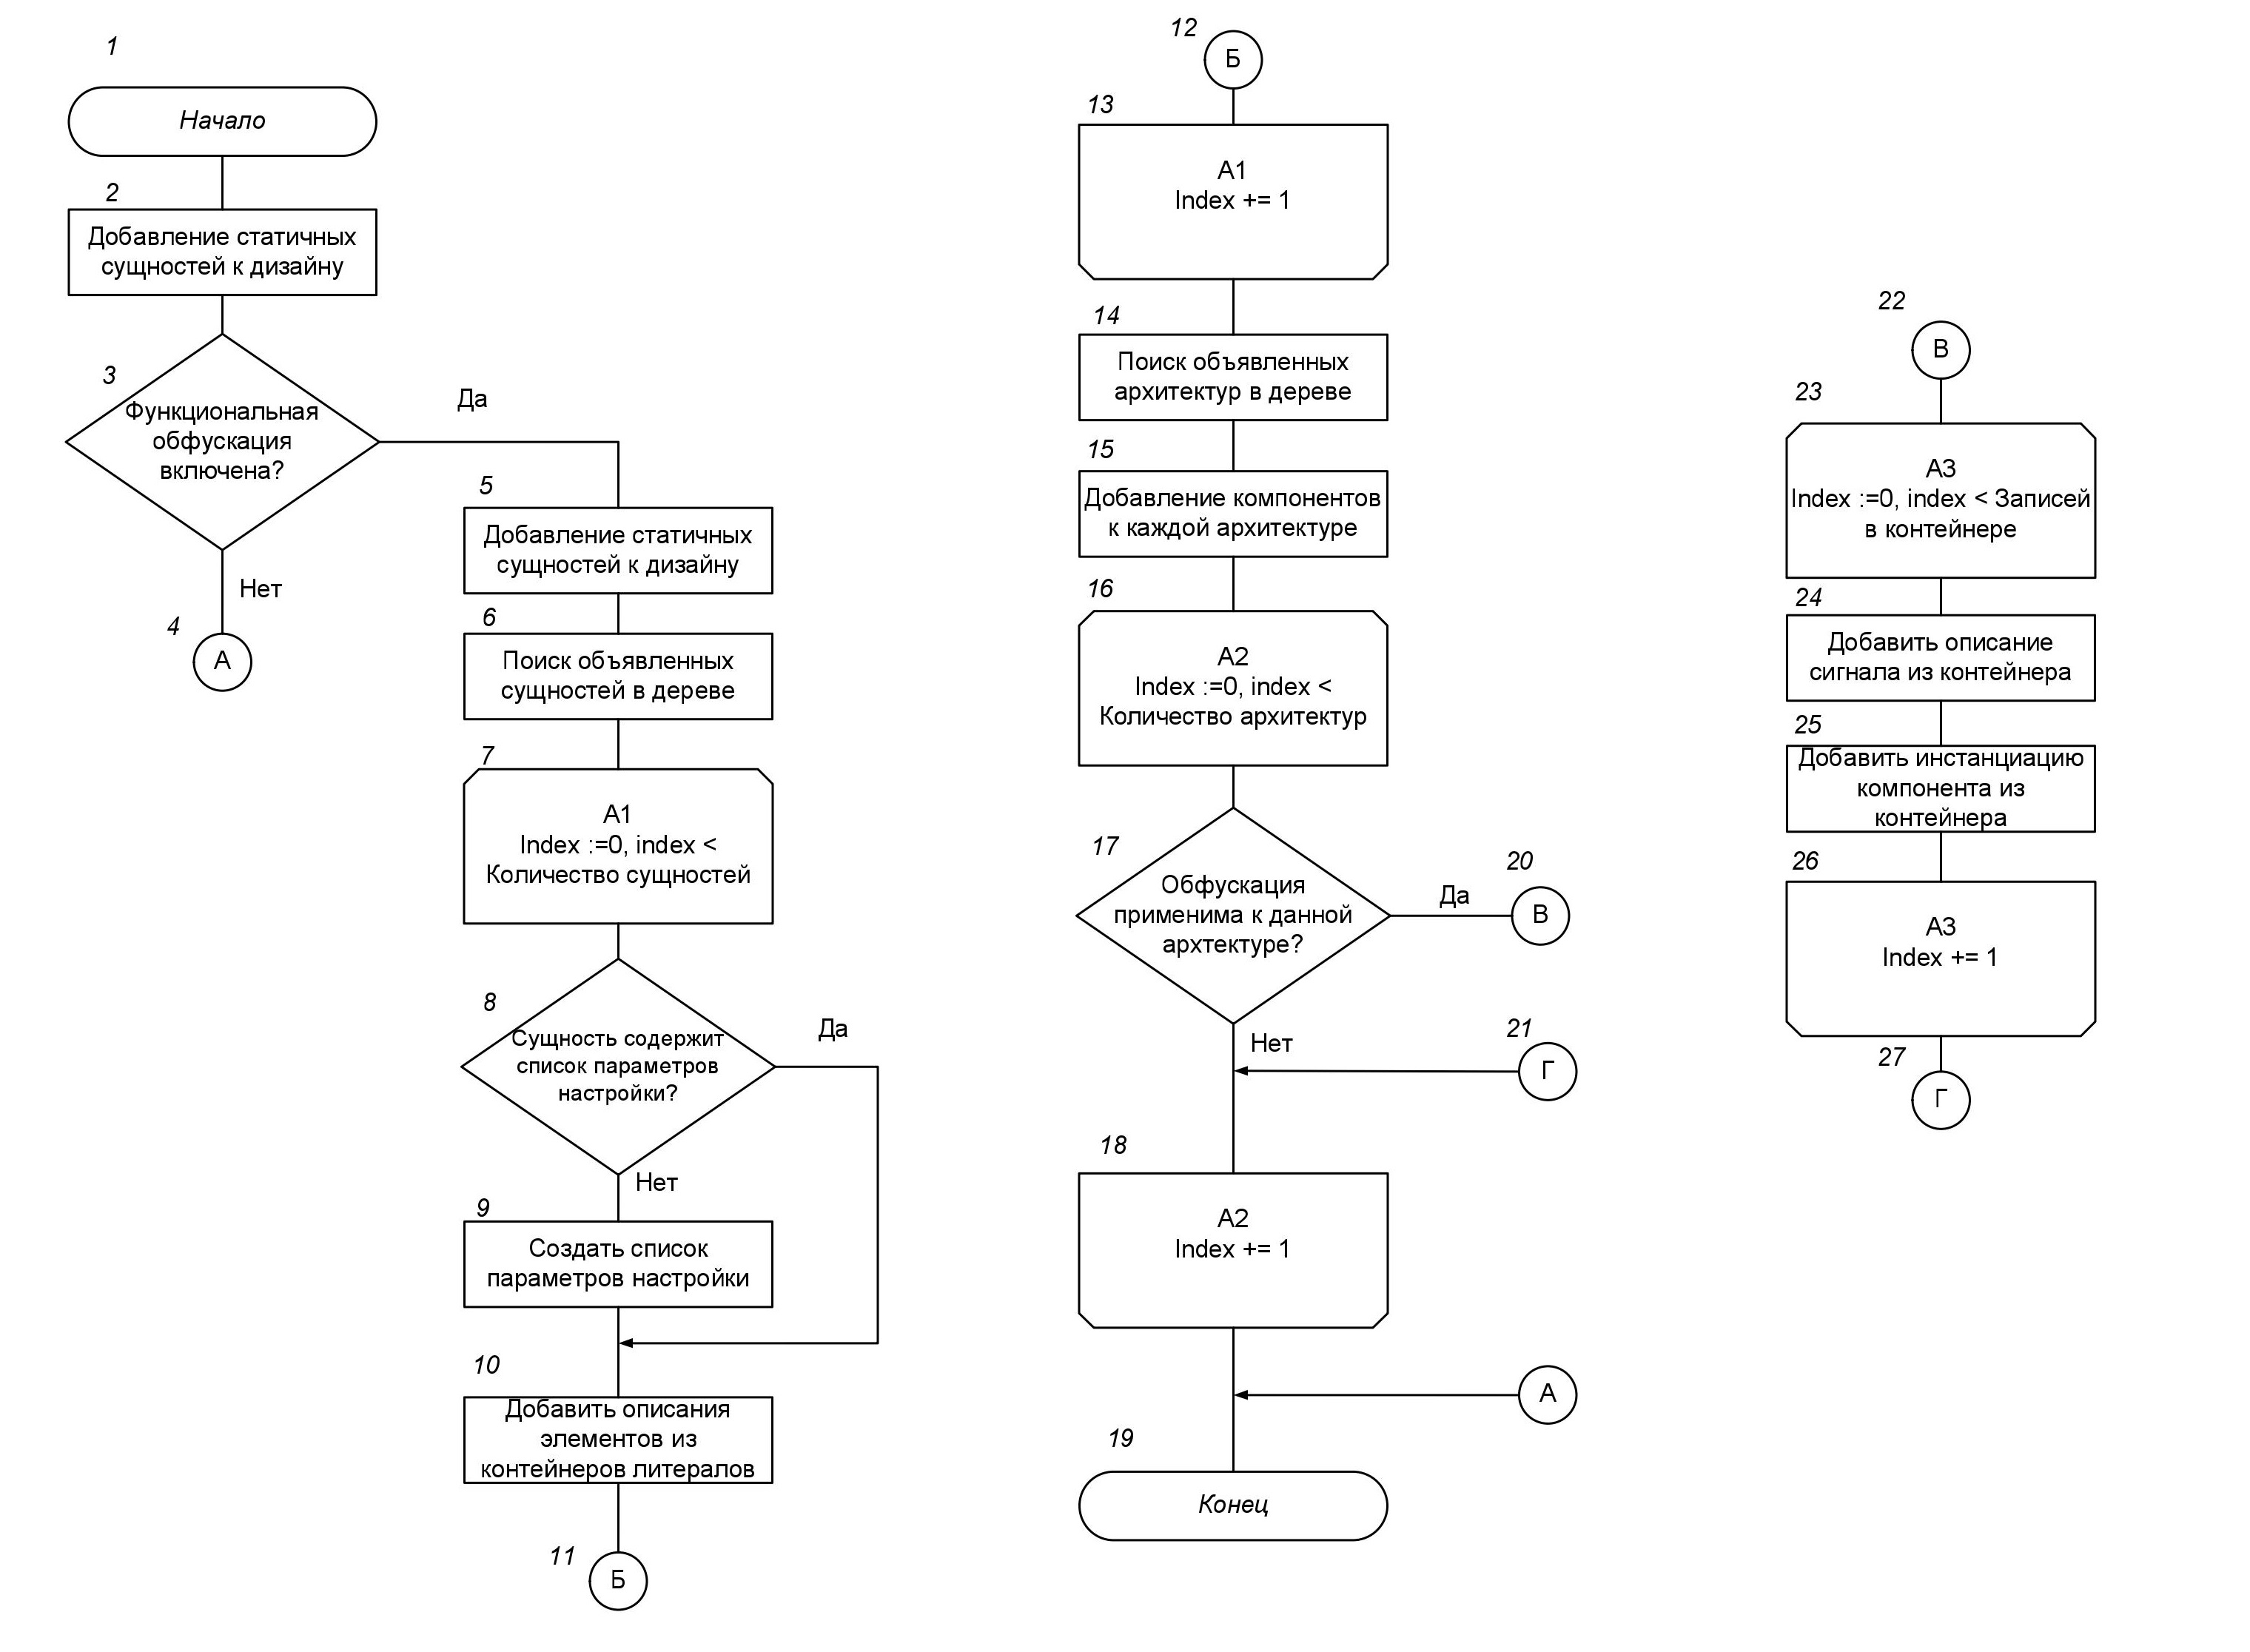
\includegraphics[scale=0.7]{obf_algo.jpg}
      \caption{ Алгоритм работы обфускатора }
      \label{fig:arch_and_mod:obf_algo}
    \end{figure}
    \end{landscape}
  }
  \clearpage

  \begin{itemize}
  \item InitializerRepository --- контейнер для хранения строковых литералов. Является статическим, содержит в себе все строковые литералы, объявленные в программе, такие как имена переменных, сигналов, процессов, архитектур. При добавлении нового литерала для него автоматически создаётся его обфусцированное соответствие:
  \begin{lstlisting}[language=Ruby, style=rubystyle,caption={Определение метода перевода класса в строку для примитива component instantiation}, label=lst:arch_and_mod:initializer_repository_add]
    def self.add identifier
      identifier = [identifier] unless identifier.is_a? Array
      @@initializers.push identifier
      @@initializers.flatten!
      @@initializers.uniq!(&:name)
      identifier.each{|i| generate_mapping_for(i)}
    end
  \end{lstlisting}


  Как видно из листинга \ref{lst:arch_and_mod:initializer_repository_add}, список литералов их соответствия являются уникальными, так как многие из них используются несколько раз(например, при объявлении архитектуры и при её окончании).
  Контейнер имеет ряд вспомогательных методов, которые используются сторонними классами для определения, существует ли соответствие для данного литерала и метод выдачи соответствия по имени литерала:


  \begin{lstlisting}[language=Ruby, style=rubystyle,caption={Вспомогательные методы контейнера}, label=lst:arch_and_mod:support_methods]
    def self.mapping_defined? identifier
      !!@@mappings[identifier]
    end

    def self.mapping_for identifier
      @@mappings[identifier]
    end
  \end{lstlisting}
  \item
  LiteralRepository --- контейнер для хранения числовых и символьных литералов. Этот контейнер имеет специфическое поведение, так как конкретные числа или символы невозможно поставить в соответствие некоторому строковому литералу. Поэтому у этих литералов существует дополнительный метод \textbf{stringified}, уникальный, для каждого типа литерала:
  \begin{enumerate}
  \item для числовых литералов:
    \begin{lstlisting}[language=Ruby, style=rubystyle,caption={Вспомогательные метод stringified для числовых литералов}, label=lst:arch_and_mod:decimal_stringified]
      def stringified
        value.to_i
      end
    \end{lstlisting}
  \item Для строковых литералов:
     \begin{lstlisting}[language=Ruby, style=rubystyle,caption={Вспомогательные метод stringified для символьных литералов}, label=lst:arch_and_mod:character_stringified]
      def stringified
        "'#{@value}'"
      end
    \end{lstlisting}
  \end{enumerate}
  Контейнер ищет соответствие по значению, возвращаемому этой функцией. Это сделано для того, чтобы избежать возможных коллизий, так как в синтаксическом анализаторе все числа и символы представлены строкой из одного символа, поэтому возможен конфликт типов при одновременном существовании в исходном коде символьных литералов '0' и '1' и соотвествующих числовых литералов.
  \item
  ConstantValueRepository --- контейнер для хранения константных значений. Этот контейнер уникален тем, что используется для функциональной обфускации: вместо генерации текстового соответствия, этот контейнер генерирует определение сигнала, которое затем добавляется в определения архитектуры и соответствующий примитив для замены оригинального значения:
  \begin{lstlisting}[language=Ruby, style=rubystyle,caption={Создание сигнала на основе значения константы}, label=lst:arch_and_mod:constant_generate_name]
    .
    .
    .
    @@signals << SignalDeclaration.new('SIGNAL', name, nil, TypeWrapper.new(literal.type, nil, true), nil)
    wires = AssociationList.new([AssociationElement.new('src', name), AssociationElement.new('q', name)])
    port_map_aspect = PortMap.new('PORT', wires)
    if literal.value == '1'
      @@statements << ComponentInstantiation.new(attr_name, 'cvg_1', nil, port_map_aspect);
    else
      @@statements << ComponentInstantiation.new(attr_name, 'cvg_2', nil, port_map_aspect);
    end
    .
    .
    .
  \end{lstlisting}
  \end{itemize}

Все 3 контейнера реализуют метод генерации случайного имени, представленный в листинге~\ref{lst:arch_and_mod:generate_name}
  \begin{lstlisting}[language=Ruby, style=rubystyle,caption={Вспомогательные метод stringified для символьных литералов}, label=lst:arch_and_mod:generate_name]
    def self.generate_random_name(size: rand(6..10), alphabet: %w{ 2 3 4 6 7 9 A C D E F G H J K M N P Q R T V W X Y Z})
      charset = alphabet
      reduced_charset = charset.reject{|x| x =~ /\d/}

      reduced_charset[rand(reduced_charset.size)] + (1...size).map{ charset.to_a[rand(charset.size)] }.join
    end
  \end{lstlisting}
Три данные класса составляют существенную часть обфускатора, так как реализуют базовый функционал, которым управляют классы-оболочки.




\subsubsection{Классы-оболочки}~реализуют базовые примитивы языка VHDL. В данном ПС представлено 32 класса, экземпляры которых при конвертации в строку представляют копию исходного кода, на основе которого был создан экземпляр. Поскольку структура проанализированного кода представляет собой дерево, классы более высшего порядка принимают в качестве аргументов классы, описывающие меньшие порядки или терминальные элементы(контейнеры литералов). Ниже представлен список классов высокого порядка:
\begin{itemize}
\item класс DesignFile является классом высшего порядка(корнем синтаксического дерева), содержащим в себе все выражения дерева. Принимает только один аргумент: набор выражений, однако играет очень важную роль в функциональной обфускации, так как именно на этом этапе добавляются дополнительные примитивы, необходимые для запутывания схемы на  уровне RTL:
  \begin{lstlisting}[language=Ruby, style=rubystyle,caption={Добавление дополнительных компонентов для функциональной обфускации}, label=lst:arch_and_mod:design_functional_obf]
    def generalize_literals
      .
      .
      .
      @statements.unshift(cvg_1, cvg_2)
      header = @statements.select {|s| s.class.name == 'EntityDeclaration'}[0].header

      unless header.is_a? Array
        header = [header]
      end
      generic_clause = nil

      append_to_header = false
      if header[0] && header[0].class.name == 'GenericClause'
        generic_clause = header[0]
      else
        generic_clause = GenericClause.new([])
        append_to_header = true
      end

      generic_clause.generics.each do |statement|
        if statement.class.name == 'SignalDeclaration'
          statement.value = statement.assigned_value
        end
      end
      statements = []

      LiteralRepository.literals.each do |literal|
        signal = SignalDeclaration.new(nil, LiteralRepository.mapping_for(literal.stringified), nil, TypeWrapper.new(literal.type, nil, true), literal.stringified)
        generic_clause.generics.unshift signal
      end

      generic_clause.generics.last.type.append_semicolon = false

      (@statements.select {|s| s.class.name == 'EntityDeclaration'}[0].header = [generic_clause,header].flatten) if append_to_header
    end
  \end{lstlisting}
\item класс EntityDeclaration содержит в себе описание структуры сущности. Сущность содержит в себе порты, константы, <<дженерики>>.
\item класс ArchitectureDeclaration описывает дизайн архитектуры. Класс принимает имя архитектуры, имя сущности, набор определений(объявления переменных, сигналов), набор операторов, и закрывающую часть(посколько VHDL имеет различные формы закрывающих конструкций). Экземпляр этого класса создаётся каждый раз, когда грамматике \textit{architecture\_declaration} находится соответствие. Кроме того, именно в этом классе добавляются дополнительные определения, созданные функциональные обфускатором:
  \begin{lstlisting}[language=Ruby, style=rubystyle,caption={Часть кода, отвечающая за функциональную обфускацию}, label=lst:arch_and_mod:declaration_functional_obf]
    class ArchitectureDeclaration

      attr_accessor :type, :identifiers
      def initialize(arch_name, entity_name, declarative_part , statement_part, closing_part)
        @name = arch_name
        @entity = entity_name
        @declarations = declarative_part
        @statements = statement_part
        @closing_part = closing_part.join(' ')
        obfuscate_literals
      end

      def obfuscate_literals
        @declarations.unshift(*ConstantValueRepository.signals)
        @statements.unshift(*ConstantValueRepository.statements)
      end
      .
      .
      .
  \end{lstlisting}
\item класс ProcessDeclaration описывает оператор процесса. Оператор процесса --- параллельный оператор, представляющий основу языка VHDL. Объявленными в процессе могут быть: объявление и тело подпрограммы, объявление типа и подтипа, объявление константы, переменной, файла, псевдонима, объявление и спецификация атрибута, объявление группы, описание use. То, что объявлено в процессе, имеет область действия (видимость), ограниченную данным процессом. Принимает в качестве параметров модифкатор процесса(POSTPONED или отсутствует), метку процесса, список чувствительности, объявления(сигналов, подпрограмм, переменных и т.д), набор операторов, закрывающую часть(аналогично классу \\ArchitectureDeclaration). Учавствует в функциональной обфускации: список чувствительности должен содержать сигналы, описанные в генераторах константных значений.
\end{itemize}

Данные классы могут использоваться и вне данного программного средства, предоставляя возможности для генерации кода на языке VHDL с помощью Ruby. Дальнейшее усовершенствование последних позволяет создать собственную библиотеку, которая будет адаптером VHDL.

Полная диаграмма компонентов представлена на рисунке \ref{fig:arch_and_mod::components}


\begin{figure}[!htb]
  \centering
  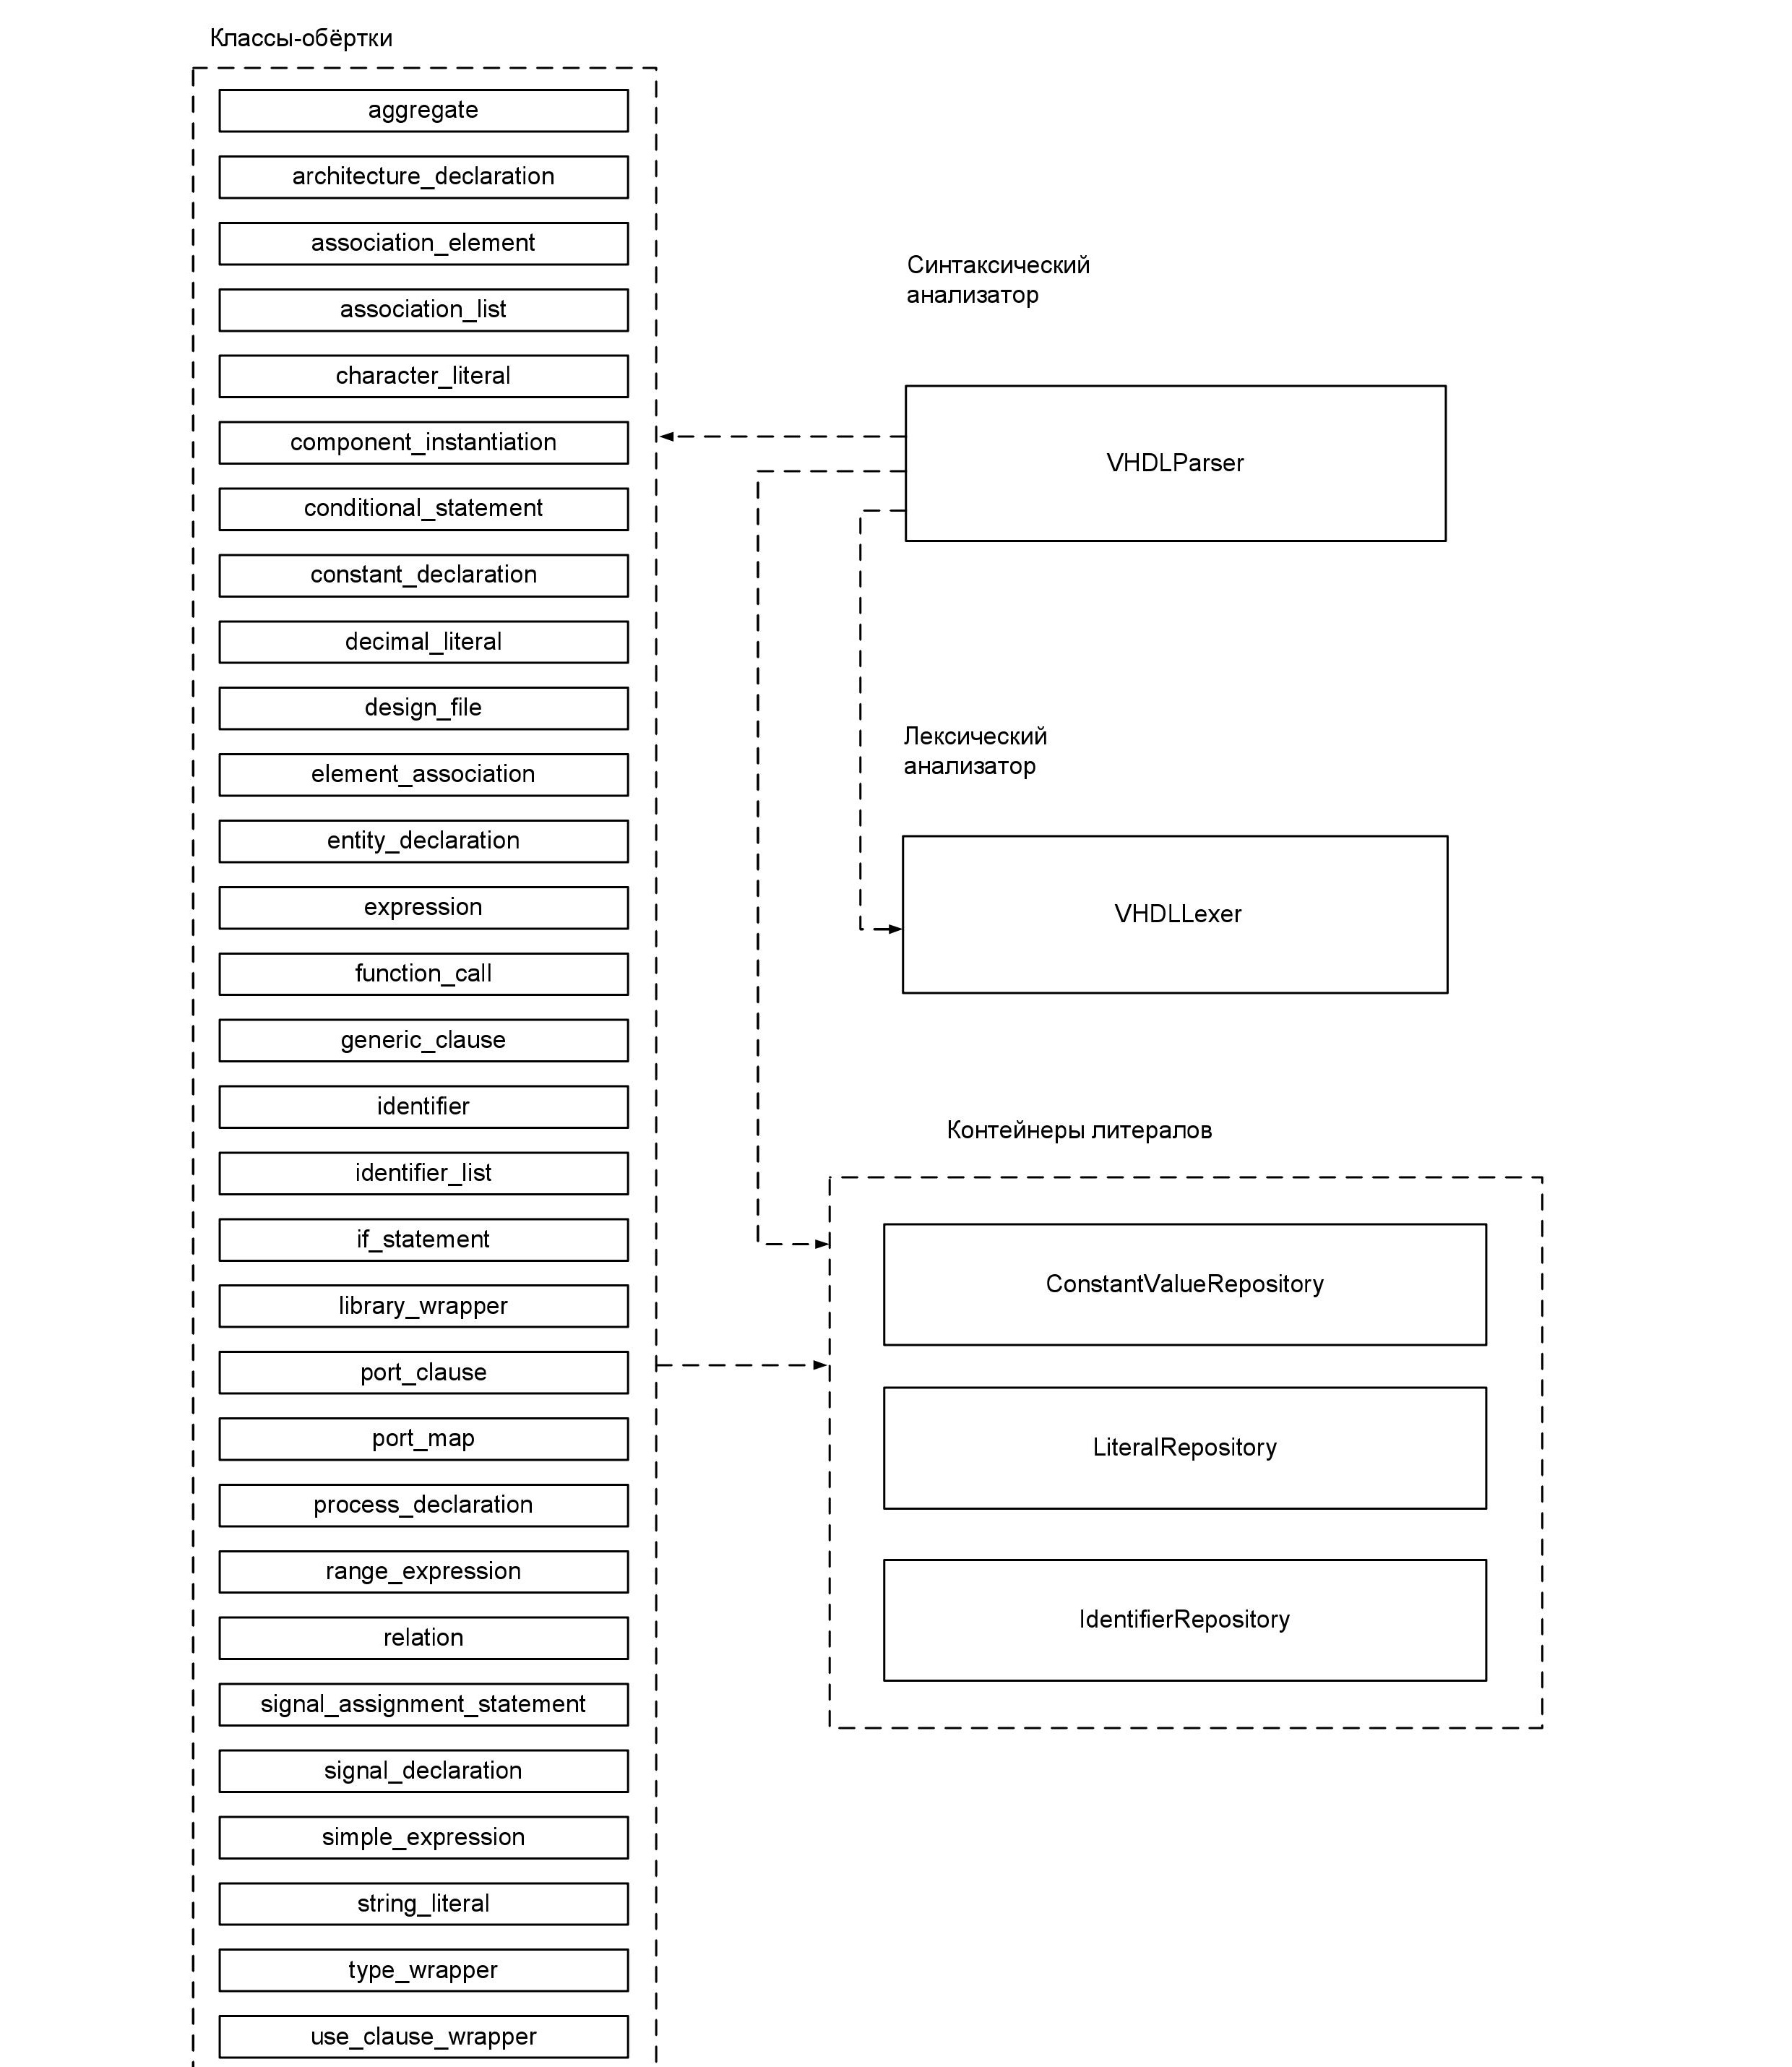
\includegraphics[scale=0.9]{components.jpg}
  \caption{ Диаграмма компонентов программного средства }
  \label{fig:arch_and_mod::components}
\end{figure}
